\section{Test}

\begin{frame}
\frametitle{Unit Testing}
\begin{itemize}
	\item Binding Parameters
	\item Incorrect Method Call
	\item Check for Correct Parameters
\end{itemize}
\end{frame}

\begin{frame}
\frametitle{Usability Test}
\begin{itemize}
	\item Field Reset
	\item Error Messages
	\item Finding History
	\item Confirmation Box
\end{itemize}
\end{frame}

\section{Discussion \& Conclusion}
\begin{frame}
\frametitle{Decisions}
\begin{itemize}
	\item Static Booking
	\item Designed for PC
	\item Hardware vs. Simulation
\end{itemize}
\end{frame}

\begin{frame}
\frametitle{Further Development}
\begin{itemize}
	\item Mobile Application
	\item Usability Test
	\item Hotspot Detection
\end{itemize}
\begin{figure}
\centering
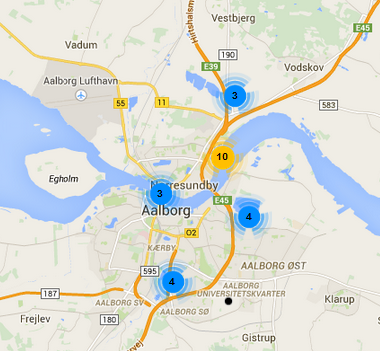
\includegraphics[scale=0.5]{MarkerClusterer}
\end{figure}
\end{frame}

\begin{frame}
\frametitle{Conclussion}
\begin{center}
	\textit{What are the requirements for a city bicycle booking and positioning system?}
\end{center}
\end{frame}

\begin{frame}
	\frametitle{Conclussion}
	\begin{center}
		\textit{How can the booking and positioning system be designed and implemented, within the context of the Internet of Things?}
	\end{center}
\end{frame}

\begin{frame}
	\frametitle{Conclussion}
	\begin{center}
		\textit{Why should the developed system be used over the currently used system?}
	\end{center}
\end{frame}

\begin{frame}
	\frametitle{Conclussion}
	\begin{center}
		\textbf{It is possible to develop a system for Aalborg Bycykel that is user friendly and manageable, within the context of the Internet of Things}
	\end{center}
\end{frame}